\documentclass[12pt]{article}

\usepackage{graphicx}
\usepackage{float}
\usepackage{xcolor}
\usepackage[normalem]{ulem}
\usepackage{cancel}
\iffalse

\fi

\setlength{\parindent}{2em}

\begin{document}
	\begin{titlepage}
	\title {Requirements Document}
	\maketitle
		\begin{center}
		SE 2XA3\\
		\author{
		Hui Chen\hspace{128pt}chenh43	
		\\*Nareshkumar Maheshkumar\hspace{35pt}maheshn 
		\\*Sam Hamel\hspace{118pt}hamels2 \\
		}

		Group E
		\end{center}
	\end{titlepage}
	
	\newpage
	\section*{Revision History}
	\begin{table}[H]
	\begin{center}
	\caption{Revision History Table}
	\begin{tabular}{|| c c c c || }\\
	\hline
	Developer & Date & Change & Revision \\
	\hline
    Hui Chen & Dec 8 2015 & \begin{tabular}[c]{@{}c@{}}Revised section 5\\ in the Test Report Document\end{tabular} & 17\\
  	\hline
	Nareshkumar Maheshkumar & Dec 8 2015 & \begin{tabular}[c]{@{}c@{}}Revised 2,3, 4.2.4, 4.2.5, 8, 9, 15 \\and 16 in the Design Document\end{tabular} & 16\\	
	\hline
  	Hui Chen & Dec 8 2015 & \begin{tabular}[c]{@{}c@{}}Revised section 2.1, 2.2.2, 2.2.3\\ in the Test Plan Document\end{tabular} & 15\\	
	\hline
	Hui Chen & Dec 8 2015 & \begin{tabular}[c]{@{}c@{}}Revised Non-functional 
	Requirements\\ in the Requirements Document \end{tabular} & 14\\
	\hline
	Nareshkumar Maheshkumar & Dec 4 2015 & \begin{tabular}[c]{@{}c@{}}Revised 3.4, 4.8 and 5.8 \\ in the Requirements Document\end{tabular} & 13\\
	\hline 
	Hui Chen & Dec 2 2015 & \begin{tabular}[c]{@{}c@{}}Revised: Fixed the numbering\\ in 3.3 and 3.4 in the \\Requirements Document\end{tabular} & 12\\
	\hline 
	Sam Hamel & Dec 2 2015 & \begin{tabular}[c]{@{}c@{}}Revised: Number the Functional \\Requirements in the \\Requirements Document\end{tabular} & 11 \\
	\hline
	Hui Chen & Oct 10 2015 & Final Edit & 10\\
	\hline
	Nareshkumar Maheshkumar & Oct 9 2015 & Final Revision & 9 \\
	\hline
	Hui Chen & Oct 9 2015 & & 8 \\
	\hline
	Sam Hamel & Oct 9 2015 & & 7 \\
	\hline
	Hui Chen & Oct 7 2015 & & 6 \\
	\hline
	Sam Hamel & Oct 7 2015 & & 5 \\
	\hline
	Nareshkumar Maheshkumar & Oct 7 2015 &	& 4	\\
	\hline
	Sam Hamel & Oct 5\&9 & & 3 \\
	\hline
	Nareshkumar Maheshkumar & Oct 3\&9 2015 & &2 \\
	\hline
	Hui Chen & Sept 29 2015& Created requirements document	& 1 \\
	\hline
	\end{tabular}
	\end{center}
	\end{table}
	
	\newpage
	\tableofcontents
	\listoffigures
	\listoftables

	\newpage
	\section{Project Drivers}
	\subsection{The purpose of the Project}
	The purpose of the project is to design and develop a Texas Hold-Em game that a person 		can play for enjoyment and improvement of their skills by getting the user acquainted 		with the rules of the game through gameplay, and by facing a challenging computer 			opponent. There are too many people who do not know the basics of the game and the goal 	is to help those who need a way to learn the game before entering their first 				professional Texas Hold-Em game, for example at a casino.
	\subsection{The Client, the Customer, and Other Stakeholders}
	\textbf{Client}
	\begin{itemize}
	\item Spencer Smith
	\end{itemize}
	\textbf{The Customer}
	\begin{itemize}
	\item Windows, Macintosh OS X, and/or Linux users
	\end{itemize}
	
	\textbf{Other Stakeholders}
	\begin{itemize}
	\item Supervisors
	\item Designers and Developers
	\item Testers
	\item End Users
	\end{itemize}

	\subsection{Users of the Product}
	The users are beginner Texas Hold-Em players who wish to learn how to play the game. It 	is assumed they have no prior knowledge of the game.  Users of any operating systems 		are accepted whether it is Windows, Macintosh OS X, or Linux users. 
	
	\section{Project Constraints}
	\subsection{Mandated Constraints}
	The current project constraint states that the product must be completed within the 		span of three months. The product shall be implemented in a GUI for simple navigation. 		The final product shall be self contained and be able to run on any major operating 		system (Windows, Macintosh, Linux). The product shall be marketed toward gamers, and/or 	poker players. The source code shall be written entirely in Java, and uses the awt and 		swing libraries from Java.
	\subsection{Naming Conventions and Definitions}
	\begin{itemize}
	\item 	Texas Hold-Em -  (also known as Texas holdem, hold 'em, or holdem) is a 					variation of the standard card game of poker.
	\item 	No limit - Game in which there is no maximum amount of money or chips that a 				player is permitted to wager.
	\item	GUI - Graphical User Interface
	\item	Heads up - A game of poker between just two players.
	\item 	Call - To accept the opponent's bet
	\item 	Raise - To make an additional bet of chips on top of the existing bet
	\item 	Check - To pass on betting
	\item	Fold - If you fold your hand in poker, you lay down your cards and stop playing 			the hand. You forfeit the round.
	\item	All in - Having all of one's chips at stake in a particular hand. Having one 				player all-in does not prevent future action by other players. Any future wager 			or portion of a previous wager that the player is not able to call goes into a 				side pot that the non-contributing player is not eligible to win.
	\end{itemize}
	\subsection{Relevant Facts and Assumptions}
	\textbf{Relevant Facts}
	\begin{itemize}
	\item	Performance will vary according to the user's computer specifications
	\item 	Gameplay experience will vary due to the random shuffle algorithm
	\end{itemize}
	\textbf{Assumptions}
	\begin{itemize}
	\item 	The users are assumed to be beginners, as our version of the game will not 					cater to professional players 
	\item 	Most users are assumed to be familiar with the operating system of their 					choosing for the usage of the product
	\item 	Most users are assumed to have the minimum memory and specifications in order 				to run the game on their personal computing device
	\end{itemize}

	\section{Functional Requirements}
	\subsection{The Scope of the Work}
	\subsubsection{Current Situation}
	There are many aspiring poker players in the world today who just wants to play a game 		of Texas Hold-Em, so in pursuit of this goal, they will need practice and experience. 	There are too many people who do not know the basics of the game and our product is meant for beginners and experienced players alike, providing experience 		without the need of monetary sacrifice. The game is built to enhance skills or to 			discover something new. The game is aimed to simplify the game as much as possible so 
	a beginner will have no problem getting into the game and they can play for enjoyment and improve their skills by getting them acquainted with the rules through gameplay and by facing a challenging computer opponent. The goal is to help the players learn the game before entering their first professional Texas Hold-Em game, for example, at a casino. 
	\subsubsection{Context of Work}
		\begin{figure}[H]
		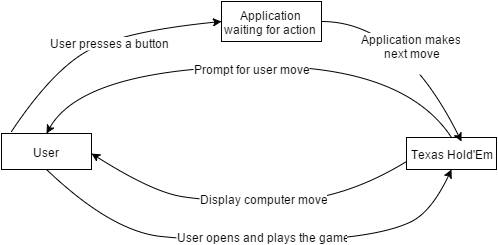
\includegraphics[scale=0.7]{ContexOfWork.jpg}
		\caption{Work Context Diagram}
		\label{fig1: Figure1}
		\end{figure}
	\subsection{Business Data Model \& Data Dictionary}
	N/A
	\subsection{The Scope of the Product}
	\subsubsection{Product Use Case}
		\begin{figure}[H]				
			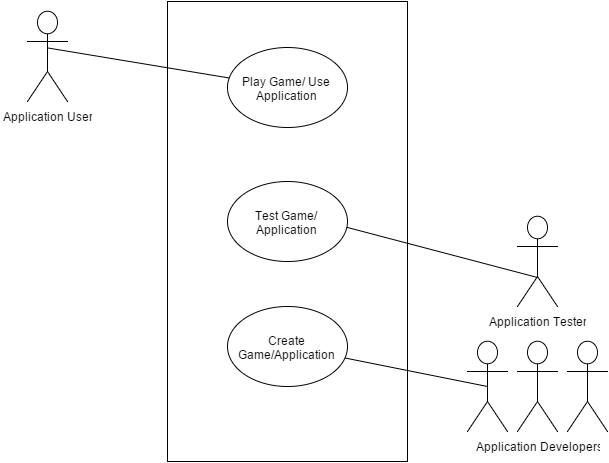
\includegraphics[scale=0.5]{UseCase.jpg}		
			\caption{Use Case Diagram}		
			\label{fig2: Figure2}		
			\end{figure}
	\subsection{Functional Requirements}
	The system shall:
	\begin{enumerate}
	\item have a help page that the user can click on to explains the rules of the game. The page should be accessible at anytime during the game, should have all the basic rules of the game, all the card hands ranked in order of strength, and extra tips and tricks.
	\item Have a GUI that the user will use to start the game and play which includes:
	\begin{itemize}
	\item a start menu with the option to view the help page, start a new game \textcolor{red}{and quit the game}
	\item a game view which shows the user their hand with, and the board cards with graphical images of the cards. It will also show the amount of chips the player and computer have, \sout{allow the user to save after each round,} and have a way to access the help page at any time via button or other means. 
	\end{itemize}
	\item have a computer program that can play Texas Hold-Em against the user, this computer program shall be able to:
	\begin{itemize}
	\item bet, raise, call, check and fold
	\item 	keep a count of the number of chips it has and the player has
	\item 	evaluate and measure hand strength
	\item	calculate the probability of winning a round based on the hand it’s given
	\item 	make actions based on the probability of winning/losing
	\end{itemize}
	\item be able to start a game, distribute cards, and monitor chip counts
	\item pit the player against a computer opponent in a match of heads up no limit 					Texas Hold-Em
	\item be able to distribute cards to the player, computer and board. The distribution of these cards should appear random and not follow any discernible pattern
	\item be able to \sout{save the game, and} end a game once either the player or the computer run out of chips
	\item \textcolor{red}{Set the default number of chips to 1000 for the player and computer} at the start of the game
	\item monitor and adjust chip count after each round
	\item end the game when either player or computer loses all their chips
	\end{enumerate}
	
	\section{Non-Functional Requirements}
	\subsection{Look and Feel Requirements}
	\textbf{Appearance Requirements} 
	\begin{itemize}
	\item 	\textcolor{red}{APP1:} The interface should be intuitive for beginners and the look should feel 					familiar to users of any operating system
	\item	\textcolor{red}{APP2:} The overall look should be clean and uncluttered
	\end{itemize}
	
	\textbf{Style Requirements}
 	\begin{itemize}
 	\item 	\textcolor{red}{STY1:}The user interface of the game should be appealing enough for the user to 					continuously want to play the game
	\end{itemize}
	\subsection{Usability and Humanity Requirements}
	\textbf{Ease of Use Requirements}
	\begin{itemize}
	\item 	\textcolor{red}{USE1:}The interface should be easy for a beginner player to start playing immediately 			after reading the rules section of the program
	\item 	\textcolor{red}{USE2:}The interface shall be intuitive and easy to navigate 
	\end{itemize}
	\textbf{Ease of Learning Requirements}
	\begin{itemize}
	\item 	\textcolor{red}{LRN1:}The rules section should be clear and concise so that someone with no prior 				knowledge can understand
	\item 	\textcolor{red}{LRN2:}The user interface should contain objects in an organized and uncluttered 					manner for ease of gameplay.
	\end{itemize}
	
	\subsection{Performance Requirements}
	\textbf{Speed requirements}
	\begin{itemize}
	\item 	\textcolor{red}{SPD1:}The game should load within 3 seconds after execution
	\item 	\textcolor{red}{SPD2:}The computer player should respond within 2 second
	\item 	\textcolor{red}{SPD3:}Button action(s) should be performed immediately
	\item 	\textcolor{red}{SPD4:}The game graphic should refresh every 1 seconds (1Hz)
	\end{itemize}	
	\textbf{Safety and Critical requirements}
	\begin{itemize}
	\item N/A
	\end{itemize}
	\textbf{Precision Requirements}
	\begin{itemize}
	\item	\textcolor{red}{PSN1:}The computer player should calculate probabilities accurate to 4 decimal places
	\item	\textcolor{red}{PSN2:}The deck shuffling should be as random as possible
	\end{itemize}
	\textbf	Reliability and Availability Requirements
	\begin{itemize}
	\item 	\textcolor{red}{RAA1:}Should be available on any operating systems (Windows, OS X, Linux)
	\item 	\textcolor{red}{RAA2:}Should be available until program closes
	\end{itemize}
	\textbf Capacity Requirement 
	\begin{itemize}
	\item 	\textcolor{red}{CAP1:}The program shall be played by a single user on a single machine
	\end{itemize}
	
	\subsection{Operational and Environmental Requirements}
	\textbf{Expected physical environment}
	\begin{itemize}
	\item	\textcolor{red}{EPE1:}The program shall be used by a single user in any environment the user wishes
	\end{itemize}
	\textbf{Expected Technological environment}
	\begin{itemize}
	\item	\textcolor{red}{ETE1:}The program shall run on any machine that has java
 	\item	\textcolor{red}{ETE2:}The program is an offline application and needs no Internet connection to run
	\end{itemize}	
	\textbf{Partner Applications}
	\begin{itemize}
	\item N/A
	\end{itemize}

	\subsection{Maintainability and Support Requirements}
	\textbf{Ease of Maintainability}
	\begin{itemize}
	\item	\textcolor{red}{EOM1:}The program does not need to be maintained once development has been completed
	\end{itemize}
	\textbf{Portability requirements}
	\begin{itemize}
	\item	\textcolor{red}{POR1:}The product is expected to run under the Windows, Apple and LINUX operating 				systems.
	\item 	\textcolor{red}{POR2:}The product should not be resource intensive
	\end{itemize}

	\subsection{Security Requirements}
	\begin{itemize}
	\item 	N/A
	\end{itemize}
	\subsection{Cultural Requirements}
	\begin{itemize}
	\item 	\textcolor{red}{CUL:}The program shall not use icons that could be considered offensive in any of 				our market countries.
	\end{itemize}
	\subsection{Legal Requirements}
	\begin{itemize}
	\item	\textcolor{red}{LEG1:}The program shall deal with only virtual currency
	\item 	\sout{The program will have a disclaimer stating that it does not advocate illegal 				gambling and should not be used as a tool to do so}
	\end{itemize}
	\section{Project Issues}
	\subsection{Open Issue}
	\begin{itemize}
	\item	Should the program include an AI that does more than read probabilities for the 			user to play against, if so how well should it play
	\item	It is difficult to test a GUI element
	\item	Is a pseudo random deck shuffler sufficient for the game or is a truly random 				method needed for shuffling the deck
	\end{itemize}
	\subsection{Off-the-Shelf Solutions}
	\begin{itemize}
	\item	There are a multitude of applications on computers and phones that allow people 			to play Texas Hold-Em against other or against a computer. 
	\item	A no limits heads up Texas Hold-Em computer algorithm has already been developed 			by the University of Alberta
	\item	Texas Hold-Em manuals already exist to help beginners learn the game quicker
	\end{itemize}
	\subsection{New Problems}
	N/A
	\subsection{Tasks}
	\begin{itemize}	
	\item 	Revise requirements document
	\item 	Create a Test Plan Revision 0 
	\item 	Demonstration for Proof of Concept
	\item 	Design Document Revision 0
	\item 	Demonstration of product Revision 0
	\item 	Document a User’s Guide 
	\item 	Generate Test Report 
	\item 	Demonstration of final product
	\item 	Revise the documentation
	\end{itemize}
	\subsection{Migration to the New Product}
	N/A
	\subsection{Risks}
	\textbf{Product Related Risks:}
	\begin{itemize}
	\item 	Computer crashes while the user is playing the game
	\item 	pseudo random deck shuffler seems to generate discernible patterns the user can 			spot
	\item 	games take too long for the user to win/lose 
	\end{itemize}
	\textbf{Contingency plans:}
	\begin{itemize}
	\item	The program will save the game after every round of hands played so that if any 			crashes happen the user can return to play from the previous hand dealt
	\item	Find a randomization algorithm with a sufficiently high complexity so that a 				human can't spot patterns
	\item	After a set duration of time, the user will be forcefully asked to fold, and if 			the game proceeds even further, the user will be asked to go all in.
	\end{itemize}
	\textbf{Production related risks:}
	\begin{itemize}
	\item	Scope of project is too large for complete development of the program in the 				time period given
	\item	proving correctness of the program will be difficult if not impossible
	\item 	Testing of Look and Feel Requirements plus Usability and Humanity requirements 				may not be viable due to lack of resources and time
	\end{itemize}
	\textbf{Contingency plans:}
	\begin{itemize}
	\item	Develop a Prototype of the program for proof of concept, if development of the 				prototype is deemed too difficult, re-evaluate the scope and requirements of 				the project 
	\item	If proof of correctness is deemed too difficult or impossible, run various 					testing methods until all developers believe the program is error free
	\item	If Testing of Look and Feel Requirements and Usability/Humanity requirements is 			not possible in the time frame given the subjective properties will be judged 				by either the developers themselves and/or by any acquaintances of said 					developers 
	\end{itemize}

	\subsection{Costs}
	There are no monetary costs involved with this projects, but about 12 weeks of 				development time be required.
	\subsection{User Documentation and Training}
	\textcolor{red}{There will be a “Game Rules” and "App Info" option in the program which will provide the user with information about the rules, key terminology and guidelines to play 		the game.} Users who 	are already familiar with their operating system should not require further training to	understand the game. 
	\subsection{Waiting Room}
	Currently there are no plans for future release of the product. In the case that a new 		release is planned, features such as online capabilities and allowing more players or 		computer opponents to play in a single game. 
	\subsection{Ideas for Solutions}
	Development of the game and GUI will be done in Eclipse.
\end{document}